% ----------------------------------------------------------------------------------------------------------------
% This .tex file (and associated .cls V3.2SP) *DOES NOT* produce:
%       1) The Permission Statement
%       2) The Conference (location) Info information
%       3) The Copyright Line with ACM data
%       4) Page numbering
% ---------------------------------------------------------------------------------------------------------------

\documentclass{acm_proc_article-sp}
\usepackage{url}
\usepackage{graphicx}
\usepackage{amssymb}
\usepackage{stackrel}
\usepackage{array}
\usepackage{amsmath}
\usepackage{verbatim}
\usepackage{multirow}
\usepackage{fancybox}
\usepackage{algorithmic}
\usepackage{algorithm}
\usepackage{blkarray}
%\usepackage{pdflscape}
%\usepackage{amsthm}
%\usepackage{fullpage}
%\usepackage{rotating}

\begin{document}

%\title{Mining Semantically Associated Itemsets from Ontology-Annotated Data}
\title{Mining Data and Ontologies Seamlessly with RDF Hypergraphs}

\numberofauthors{5}
\author{
% one 'row of three' or two rows (consisting of one row of three and a second row of one, two or three).
% 1st. author
\alignauthor
Haishan Liu\\
       \affaddr{University of Oregon}\\
       \affaddr{Eugene, OR, 97403, USA}\\
       \email{ahoyleo@cs.uoregon.edu}
% 2nd. author
\alignauthor Dejing Dou\\
       \affaddr{University of Oregon}\\
       \affaddr{Eugene, OR, 97403, USA}\\
       \email{dou@cs.uoregon.edu}
% 3rd. author
\alignauthor Paea LePendu\\
       \affaddr{Stanford University}\\
       \affaddr{Stanford, CA, 94305, USA}\\
       \email{plependu@stanford.edu}
\and  % use '\and' if you need 'another row' of author names
% 4th. author
\alignauthor Ruoming Jin\\
       \affaddr{Kent State University}\\
       \affaddr{Kent, OH, 44242, USA}\\
       \email{jin@cs.kent.edu}
\alignauthor Nigam Shah\\
       \affaddr{Stanford University}\\
       \affaddr{Stanford, CA, 94305, USA}\\
       \email{nigam@stanford.edu}
}
\date{20 January 2012}

\maketitle
\begin{abstract}
In this paper, we address an interesting data mining problem of finding semantically associated itemsets (i.e., items connected via indirect links) on ontology-annotated datasets. Semantically rich datasets, such as those annotated by formal ontologies and represented in RDF or OWL, can be viewed as datasets embedded with domain knowledge. This new standard of representation provides a unique opportunity to mine the data and domain knowledge simultaneously. In this paper, we develop a way to represent both data and ontology in a unified graph representation, and we propose to use random walk with restart to efficiently calculate the similarity between items so as to determine their associations from very large size of data and ontologies.
We show the proposed method is indeed capable of capturing semantically associated itemsets while seamlessly incorporate domain knowledge defined in ontologies through experiments performed with real life data and ontologies. The semantically associated itemsets discovered in our experiment is promising to provide valuable insights on interrelationship between medical concepts and other domain specific ones.

\end{abstract}

%\category{H.2.8}{Database Management}{Data Mining}
%\terms{Algorithms, Theory}

\keywords{Semantic Data Mining, Random Walk, Semantically Associated Itemset} % NOT required for Proceedings

%\theoremstyle{definition}
\newtheorem{myexp}{Example}[section]
\newtheorem{mydef}{Definition}[section]
\newtheorem{mythm}{Theorem}[section]
\newtheorem{mylem}{Lemma}[section]
\section{Introduction}
\label{sec:intro}

Researchers around the world are linking more and more data to ontologies which are formal specification of concepts and relationships in various domains. Formal ontologies have been extensively developed and harnessed in scientific research, particularly in biomedical research. Knowledge evolves rapidly in biomedicine and has promoted the creation and use of ontologies to advance scientific progress.  Besides the size of data increases exponentially, an increasing number of ``large" biomedical ontologies are developed. Prominent examples of this effort include the Gene Ontology (GO)~\cite{GO} and the Unified Medical Language System (UMLS)~\cite{UMLS}. Over 300 ontologies have been loaded into the National Center of Biomedical Ontology (NCBO) BioPortal library at Stanford~\cite{Noy2009}, specifying more than 5.6 million terms in the biomedical domain.

There are two major challenges facing researchers when it comes to mining large sets of biomedical ontologies and data. The first is to leverage both ontologies and data in a systematic and scalable way. The second is to deal with errors in both ontologies and data since neither of them is perfect in reality. Previous research has not been sufficient to address these challenges. For example, some approaches have utilized ontologies in data mining, but usually only a small portion of ontologies is used (typically the subsumption relationship) on very few tasks (most often concept aggregation). On the other hand, limited attempts have been made to check errors in large ontologies. Traditional approaches to sanitize knowledge bases by using an inference engine for logic reasoning and consistency checking is hard to scale.

With the increasing amount of ontology-annotated data, new possibilities are opened up for both data mining and ontology development. Therefore an emerging research direction, which we call \textit{semantic data mining}, focuses on drawing insights from both domain knowledge and data in a systematic way. It aims at bringing domain knowledge seamlessly into the data mining process, and helps improve the quality of pattern discovered in a noisy environment. It also benefits the ontologies by utilizing empirical substantiation from data to either bolster a priori ontological assertions, or detect potential errors therein.

Semantic data mining leverages links between entities defined by ontologies---via annotations---to the mining algorithms explicitly in a unified model. This requires traversing links across the ontologies to infer implicit inter-connections among the data. Graph techniques fit this research nicely because both domain knowledge and semantically rich datasets can be represented as graphs. For example, OWL~\cite{OWL} is the standard ontology language built on RDF. Inheriting the graph nature of RDF, any collection of OWL ontologies or RDF data is an RDF Graph~\cite{GraphModelRDF}. In fact, many semantically rich datasets of interest today, such as DBpedia,  are best described as a linked collection, or a graph, of interrelated objects~\cite{LinkMiningGetoor}. These graphs may represent both homogeneous networks and heterogeneous networks.

Hence, our semantic data mining approach is inspired by a combination of graph representation~\cite{CheinMugnier08}, hypergraphs~\cite{Zhou06learningwith}, and random walks~\cite{Fouss06random-walkcomputation, Zhou:2009:GCB:1687627.1687709}. This paper extends our previous work that implements a hypergraph-based approach to learn associations from interlinked data (without ontologies)~\cite{LiuEtal11}. The RDF hypergraph representation proposed by Hayes et al.~\cite{GraphModelRDF} is a key innovation which connects data and ontologies. We adopt this representation in our approach because properties in RDF triples can be represented as first class objects among all interrelated objects, enabling us to embed both the ontology and the data together and to serialize it into a bipartite graph representation for scalable processing.

In RDF hypergraphs, we use random walk with restart to efficiently calculate the similarity between concepts to determine their associations from large set of data and ontologies. Traditional association mining relies on co-frequencies of items (concepts) within transactions~\cite{Agrawal94}. We look one step further to find indirectly associated items (concepts). This extension has far reaching applications in biomedicine. For instance, consider a simple scenario illustrated by Swanson~\cite{swanson87} years ago while studying Raynauld's syndrome. He noticed that the literature discussed Raynauld's syndrome ($Z$), a peripheral circulatory disease, together with certain changes of blood in human body ($Y$); and, separately, the consumption of dietary fish oil ($X$) was also linked in the literature to similar blood changes.  But fish oil and Raynauld's syndrome were never linked directly in any previous publications.  Swanson reasoned (correctly) that fish oil could potentially be used to treat Raynauld's syndrome, i.e., $X\rightsquigarrow Y \rightsquigarrow Z$. We call such indirect associations, $(X,Z)$, \emph{semantic associations}.

We evaluate the effectiveness of the results on large real-world biomedical data and ontologies. We show the proposed method is indeed capable of capturing semantic (indirect) associations while seamlessly incorporate domain knowledge defined in formal ontologies. We also show that our data mining methods can discover misinformation in biomedical ontologies. Our work makes the following main contributions: First, we employ a RDF hypergraph representation to capture both semantics of ontologies and data. We can weight each hyperedge so that certain links (such as \emph{is\_a} or \emph{may\_treat} relationships) can carry appropriate strength.  Next, we serialize the hypergraph and weighted hyperedges into a bipartite representation for efficient processing. Then, we implement highly efficient and scalable random walks with restart over the bipartite graph to generate semantic associations, including associations that may not necessarily be co-frequent. The discovered semantic associations can be used to detect potential errors in biomedical ontologies.


\section{Related Work}
\subsection{Ontologies and Data Mining}
Using formal ontologies to annotate data has become increasingly popular in biomedical domains. For instance, in genetics, researchers curate literature to generate ontology-annotated data for different species of model organisms by linking specific proteins to various classes in the Gene Ontology (GO~\cite{GO}). These publicly available GO annotation databases make enrichment analysis possible, which enables researchers to functionally profile sets of interesting genes identified by microarray experiments~\cite{Khatri2005}.  At Stanford, the National Center for Biomedical Ontology (NCBO) annotates large volumes of biomedical text for search and mining~\cite{RI} and has been used, for instance, to profile disease research~\cite{Liu2012}.  Finally, millions of patient electronic health records are being annotated using medical ontologies like SNOMED-CT in efforts to advance patient healthcare~\cite{OMOP}.

In general domains, Staab and Hotho~\cite{StaabH03} were one of the earliest to utilize the idea of mapping terms in text to classes in an ontology and they essentially use the ontology to aggregate data and thus reduce feature dimensionality during clustering.  Adryan et al.~\cite{Adryan2004} enable cluster visualization for gene expression data by navigating various levels of Gene Ontology hierarchy.  %Shen et al.~\cite{Shen2006Ont} use the ontology to check for consistency of association rules. 
Wen et al.~\cite{Wen2007Ont} take into consideration the ontology hierarchy to offset biases toward overly-general terms in text mining.

\subsection{Graphs in Mining RDF and Ontologies}

RDF data and OWL ontologies can be represented as graphs for data mining. Lin et al.~\cite{Lin2011Learning} treat the RDF triple store as a datasource during mining and develop Relational Bayesian Classifiers (RBCs) that aggregate SPARQL queries. Kiefer et al.~\cite{Kiefer2008Adding} extend the SPARQL query language to enable creating and working with the data mining model. Similarly, Bicer et al.~\cite{Bicer2011Relational} define kernel machines over RDF data where features are constructed by ILP-based dynamic propositionalization. In each case, RDF is merely a data model, paying little attention to the use of domain-specific knowledge in related ontologies.

Recently, a promising graph-based approach to represent and mine ontologies and data together is Heterogeneous Information Networks (HIN) developed by Sun et al.~\cite{SunHYYW11, SunNHYYY12}. HIN leverages semantics of various types of nodes and links in a network for the graph and network mining tasks. Since ontologies and annotated data can be treated as a large graph of concepts and entities linked with different type of relationships, there should be a way to represent certain relationships and semantics (e.g., class subsumption) of ontologies and data in HIN. However, considering many biomedical ontologies are large, manually representing them in heterogeneous information networks is not practical. It is not easy to build an automatic translator from OWL ontologies to HIN either. We prefer RDF Hypergraphs because the RDF syntax of OWL ontologies and data makes it much easier to automatically transform existing biomedical ontologies and their annotated data into RDF hypergraphs. 
%\section{Related Work}
\label{sec:related}
In this section, we discusses the current state of the effort to incorporate domain knowledge especially formal ontologies in data mining. In addition, we also describe the various formalisms proposed in the literature to use graphs in tackling Semantic Web and data mining problems.

%\subsection{Ontologies in Data Mining}
%Domain knowledge relates to information about a specific domain or data that is collected from previous systems or documentation, or elicited from domain experts.

%We first highlight a selection of studies that aims at exploring domain knowledge encoded in formal ontologies in data mining. Domain knowledge can affect data mining systems in at least two ways. First, it makes patterns more visible by generalizing attribute values; and second, it often reduces the search space by introducing constraints and heuristics.

%Staab and Hotho~\cite{StaabH03} describe an ontology-based text clustering approach. They develop a preprocessing method, called COSA, one of the earliest to utilize the idea of mapping terms in the text to concept in the ontology. By mapping terms to concepts, it essentially aggregates terms and reduces the dimensionality. Adryan et al.~\cite{Adryan2004} developed a system called GO-Cluster which uses the tree structure of the Gene Ontology database as a framework for numerical clustering, and thus allowing a simple visualization of gene expression data at various levels of the ontology tree. Shen et al.~\cite{Shen2006Ont} proposed a method of association rules retrieval that is based on ontology and Semantic Web. Ontological semantics and reasoning can be used for sharing and consistency checking of discovered association rules. Wen et al.~\cite{Wen2007Ont} propose a technique for concept frequency re-weighing to solve the problem in text mining that a document is often biased towards class-independent ``general" words while short of class-specific ``core" words. The proposed method takes into consideration the concept hierarchy defined in the domain ontology.

More recent studies have focused on developing scalable and incremental data mining systems by tapping on the distributed characteristics of OWL and RDF. Kiefer et al~\cite{Kiefer2008Adding} propose to perform statistical learning and inference on RDF data by directly extending the SPARQL query language that enables creating and working with a data mining model in SPARQL. Lin et al.~\cite{Lin2011Learning} describe an approach to learning Relational Bayesian Classifiers (RBCs) from RDF data by querying statistics of data through the SPARQL endpoint thus allowing the storage to be decentralized. They also establish the conditions under which the RBC models can be incrementally learned in response to changes of RDF data.

%However, previous ontology-based data mining approaches treat the data and ontologies separately and handle the tasks in much smaller scale especially respect to the number ontological concepts in real life ontology-annotated data we deal with in this paper.


\subsection{Graph-based formalism in Semantic Web and Data Mining}

Given the fact that OWL ontologies and RDF documents in Semantic Web have a graph nature, we hope to employ a graph-based formalism to represent annotated data so that the ontologies and data can be combined for mining in a systematic manner. Hayes has established that RDF can be also represented as hypergraphs (bipartite graphs)~\cite{GraphModelRDF}. The closely related ones to this paper are random work and hypergraphs in a number of data mining systems.
%Various quantities derived from random walk has been proposed to model the relevance, or similarity between entities in a graph. Fouss et al.~\cite{Fouss06random-walkcomputation} compare twelve scoring algorithms based on graph representation of the database to perform collaborative movie recommendation. Pan et al.~\cite{Pan} develop a similarity measure based on random walk steady state probability to discover correlation between multimedia objects containing data of various modalities.
Yen et al.~\cite{Yen05clusteringusing} introduce a new k-means clustering algorithm utilizing the random walk average commute time distance. Zhou et al.~\cite{Zhou:2009:GCB:1687627.1687709} presented a unified framework based on neighborhood random walk to integrate structural and attribute similarities for graph clustering. The concept of random walk is extended to hypergraph~\cite{Zhou06learningwith}. Tian et al.~\cite{Tian09} propose a hypergraph-based learning algorithm to classify gene expression data. They also take into account previous knowledge by modeling the knowledge as regularization terms in the optimization problem.
In our previous work, the authors have developed a hypergraph-based method for discovering semantically associated itemsets~\cite{LiuEtal11}. Although the results are promising and interesting to domain experts, we have only utilized the data graphs for association mining but not the rich semantics of ontologies. In this paper,  we presents a Semantic Data Mining framework which will draw insights from both ontology and data in a systematic and efficient way.


\section{Method}
\label{sec:method}
The synergy between ontologies and data mining can be achieved by employing the RDF model given the fact that RDF allows a combined specification of both schema information and data structured under the schema. In light of Hayes et al's proposal to represent RDF as hypergraphs~\cite{GraphModelRDF}, we develop a set of rules to represent data in transactional tables as hypergraphs or bipartite graphs with minimal loss of semantics. We then propose a novel way to combine the graph representations of data and domain knowledge encoded in ontologies as a unified information source from which valuable insights can be drawn upon.

\subsection{Graph Representation for Ontologies}
The Web Ontology Language (OWL~\cite{OWL}) is the W3C's standard for representing knowledge in the Semantic Web~\cite{Berners-Lee01}---a giant semantic network that spans the entire Internet. OWL ontologies can be used along with information written in RDF, and OWL ontologies themselves are primarily exchanged as RDF documents, too. RDF's abstract triple syntax has a graph nature. The RDF graph is defined as a set of RDF triples and can be visualized as a \emph{directed labeled graph} (DG) as follows:
\begin{center}\ovalbox{subject} $\stackbin[]{predicate}{\xrightarrow{\hspace*{2cm}}}$ \ovalbox{object}\;.\end{center}

One disadvantage of DG is that it makes an artificial distinction between resources and properties, which leads to incongruous representations. Consider the RDF statements in the following example. $\langle$ \texttt{Alice collaborateWith Bob}$\rangle$, $\langle$ \texttt{Bob coauthorWith Charlie}$\rangle$, $\langle$ \texttt{coauthorWith subPropertyOf collaborationWith}$\rangle$. From the first two statements, \texttt{Alice, Bob} and \texttt{Charlie} can be represented in a DG as nodes connected by edges \texttt{collaborativeWith} and \texttt{\texttt{coauthorWith}} respectively. However, from the last statement, to express the relationship between \texttt{collaborativeWith} and \texttt{coauthorWith}, these concepts have to be represented as nodes themselves. Representing this set of statements in DG inevitably separates the information into two inconsistent subgraphs, making it difficult for graph-based methods to utilize the information in a holistic and systematic manner.

To overcome the inconsistency, Hayes et al.~\cite{GraphModelRDF} proposed to model RDF as a \emph{hypergraph}. A hypergraph~\cite{Hypergraph} is a generalization of a traditional graph where edges, called hyperedges, can connect more than two vertices. If each edge in a hypergraph covers the same number of nodes, it is called $r$-uniform hypergraph, $r$ being the number of nodes on each edge. Any RDF graph can be represented by a simple ordered 3-uniform hypergraph, in which an RDF triple corresponds to a hyperedge, with incident nodes being the subject, predicate and object from the triple. In this way, both meta-data and data level statements can be integrated in a consistent graph representation.

Formally, a hypergraph $HG = (V,E)$, is a pair in which $V$ is the vertex set and $E$ is the hyperedge set where each $e \in E$ is a subset of $V$. A weighted hypergraph is a hypergraph that has a positive number $w(e)$ associated with each hyperedge $e$; called the weight of hyperedge $e$: Denote a weighted hypergraph by $G = (V,E,w)$. Furthermore, A hypergraph $HG = (V, E)$ can be transformed to an \emph{bipartite graph} $BG$ as follows: the node sets $V$ and $E$ be the two parts of $BG$, and $(v_1, e_1)$ is connected with an edge if and only if vertex $v_1$ is contained in the hyperedge $e_1$ in $HG$. In other words, the incidence matrix of $HG$ can be viewed as the node adjacency (biadjacency) matrix of the bipartite graph.

BG have many desirable properties for developing intuitive mining algorithms because they turn hypergraphs into a simple form so that many algorithms designed on simple graphs can be readily applied. Therefore, we propose to use bipartite graphs to represent domain knowledge and data expressed in RDF.

\subsection{Graph representation for Ontology-annotated Data}
There already exist methods for transforming data, such as those in relation databases, into RDF~\cite{RDB2RDF}. An ontology-annotation, as we see it, is a binary value representing whether some ontological concept (or class) is associated with some entity.  Often, this means that some concept appears in some document and thus the ontology serves to index the document with related concepts~\cite{RI}.  Thus, we can think of ontology-annotations as a table, with each row representing an entity (e.g., a document), and each column is a class from some ontology.  Cells having a ``1'' denotes that the document \emph{mentions} the term defined by the class.  RDF can be seen as a sparse matrix representation of this data (Table~\ref{tbl:binary-rel}).  This idea can be easily extended to nominal-valued tables as well, or with other relationships besides \emph{mentions} as we illustrate when discussing ontologies as bipartite graphs in the next section.
\begin{table}[ht]
\begin{minipage}[b]{0.38\linewidth}\begin{flushright}
\begin{tabular}{ c | c | c | c |}
\cline{2-4}
	~   & $f_1$	    & $\cdots$  & $f_n$   \\
\cline{2-4}
$r_1:$	&  0  	& $\cdots$   &    1  \\
\cline{2-4}
$\vdots$& $\vdots$  & $\ddots$  & $\vdots$\\
\cline{2-4}
$r_m:$	&  1  	& $\cdots$   &    0  \\
\cline{2-4}
\end{tabular}
\end{flushright}
\end{minipage}
\hfill
\begin{minipage}[b]{0.4\linewidth}
\begin{tabular}{c c c}
\emph{s}&   \emph{p}&  \emph{o}\\
\texttt{<$r_1$}   &    \texttt{mentions}   &  \texttt{$f_n$>}\\
\texttt{<$r_m$}   &    \texttt{mentions}   &  \texttt{$f_1$>}\\
\end{tabular}
\end{minipage}
\begin{minipage}[c]{0.4\linewidth}\centering
\vspace{0.2cm}\hspace{1.5cm}(A)
\end{minipage}
\begin{minipage}[c]{0.4\linewidth}\centering
\hspace{2.6cm}(B)
\end{minipage}
\caption{\label{tbl:binary-rel} Ontology-annotated data (A) is a feature matrix attributing classes from ontologies, $f_i$, to entities such as documents, $r_j$, that is easily represented in sparse matrix form using RDF statements (B).}
\end{table}

\subsection{Combined Graph Representation for Ontologies and Data}
In order to facilitate the synergy between data and domain knowledge in a mining framework, information from both sources needs to be first combined. This is achieved by the process called \emph{semantic annotation}. Semantic annotation aims at assigning formal semantic descriptions to the basic element of data, and it is crucial in realizing semantic data mining by bridging formal semantics in domain knowledge with data. If data is annotated, a unified graph incorporating information from both data and ontologies can be created. Data mining algorithms dealing with such unified graph representation can enjoy the benefit of a seamless integration of domain knowledge. The following example demonstrates the combination of an ontology graph and a data graph.

Figure~\ref{fig:onto-and-data} (A) shows a simple ontology with only subsumption relationships defined for five concepts (A--B). Figure~\ref{fig:onto-and-data} (B) is a binary-valued RDB table in the same domain with the set of concepts (A--B) being features. We use the same concept labels in the ontology and the RDB table because we assume the mapping between the ontology nodes and the table features are pre-assigned manually or established by automatic annotation. Figure~\ref{fig:hypergraph-combined} (B) shows the RDF statements derived from both the ontology and the RDB table. Figure~\ref{fig:hypergraph-combined} (A) demonstrates the combined RDF bipartite graph.

\begin{figure*}[tbh]
\begin{minipage}[c]{.4\textwidth}\centering
\includegraphics[width=.5\linewidth]{fig/simple-onto.eps}
\end{minipage}
\begin{minipage}[c]{.25\textwidth}\centering
    \begin{tabular}{ c | c | c | c | c | c |}
    \cline{2-6}
    	~ & A & B & C & D & E\\
    \cline{2-6}
    $A:$& 0 & 0 & 1 & 0 & 0 \\
    \cline{2-6}
    $B:$& 0 & 0 & 1 & 0 & 0 \\
    \cline{2-6}
    $C:$& 0 & 0 & 0 & 0 & 1 \\
    \cline{2-6}
    $D:$& 0 & 0 & 0 & 0 & 1 \\
    \cline{2-6}
    $E:$& 0 & 0 & 0 & 0 & 0 \\
    \cline{2-6}
    \end{tabular}
\end{minipage}
\begin{minipage}[c]{.25\textwidth}\centering
    \begin{tabular}{ c | c | c | c | c | c |}
    \cline{2-6}
    	~ & A & B & C & D & E\\
    \cline{2-6}
    $r_1:$& 1 & 1 & 0 & 0 & 0 \\
    \cline{2-6}
    $r_2:$& 1 & 1 & 1 & 0 & 0 \\
    \cline{2-6}
    $r_3:$& 0 & 1 & 1 & 0 & 0 \\
    \cline{2-6}
    $r_3:$& 0 & 0 & 0 & 1 & 0 \\
    \cline{2-6}
    \end{tabular}
\end{minipage}
\begin{minipage}[c]{0.4\linewidth}\centering
(A)
\end{minipage}
\begin{minipage}[c]{0.25\linewidth}\centering
(B)
\end{minipage}
\begin{minipage}[c]{0.25\linewidth}\centering
(C)
\end{minipage}
\caption{\label{fig:onto-and-data} Five concepts (\emph{A--E}) are represented visually as a hierarchy (A) and also as a a hypergraph using the binary feature matrix (B), where a ``1'' denotes \emph{rdfs:subClassOf}, which is similar to the ontology-annotated data (C), where ``1'' denotes \emph{mentions}.}
\end{figure*}

\begin{figure*}[tbh]
\begin{center}
\begin{tabular}{c  c}
\multirow{12}{*}{\includegraphics[width=.45\textwidth]{fig/hypergraph_mining.eps}} & \emph{~~~~~~~s \hfill p\hfill o~~~}\\
& $s_1$:~~~\texttt{<A>~~<subClassOf>~~<C>}\\
& $s_2$:~~~\texttt{<B>~~<subClassOf>~~<C>}\\
& $s_3$:~~~\texttt{<C>~~<subClassOf>~~<E>}\\
& $s_4$:~~~\texttt{<D>~~<subClassOf>~~<E>}\\
& \\
& $s_5$:~~~\texttt{<r1>\;~~<mentions>\;~~<A>}\\
& $s_6$:~~~\texttt{<r1>\;~~<mentions>\;~~<B>}\\
& $s_7$:~~~\texttt{<r2>\;~~<mentions>\;~~<A>}\\
& $s_8$:~~~\texttt{<r2>\;~~<mentions>\;~~<B>}\\
& $s_9$:~~~\texttt{<r2>\;~~<mentions>\;~~<C>}\\
& $s_{10}$:~~\texttt{<r3>\;~~<mentions>\;~~<B>}\\
& $s_{11}$:~~\texttt{<r3>\;~~<mentions>\;~~<C>}\\
& $s_{12}$:~~\texttt{<r4>\;~~<mentions>\;~~<D>}\\
& \\
& \\
& \\
& \\
(A) & (B)\\
\end{tabular}
\end{center}
\caption{\label{fig:hypergraph-combined} The RDF bipartite graph representation (A) easily combines both the ontology-annotated data with the ontological relationships (B) based on the information described in Figure~\ref{fig:onto-and-data}.}
\end{figure*}

Formally, the RDF bipartite graph as a combined representation for both data and ontologies is defined as $G=\langle V_v \cup V_s, E \rangle$, where $V_v$ denotes \emph{value nodes} corresponding to components of RDF statements (i.e., subject, predicate, or object), and $V_s$ denotes \emph{statement nodes} corresponding to RDF statements. More specifically, statement nodes can be further divided according to whether they are from data or ontology, i.e., $V_s=V_d \cup V_o$; Value nodes can be divided according to whether they represent rows (records) or columns (attributes) in data, \i.e., $V_d=V_r \cup V_a$. The graph $G$ can be represented in a biadjacency matrix $\mathbf{M}$, where $\mathbf{M}(i,j)$ is non-zero if there is an edge between $\langle V_{v_i}, V_{s_j} \rangle$. For an unweighted graph, the value can be 0/1, and for a weighted graph, any non-negative value. Weights assigned to different paths in the graph are used to distinguish various semantic types or relationships (properties) from the ontology and data, such as class subsumption, ``part\_of", and other general or domain--specific properties.
 
For example, Figure~\ref{fig:biadjacency-matrices} shows the biadjacency matrices $\mathbf{M}_d$ and $\mathbf{M}_o$ for the data and ontology part of the RDF bipartite graph respectively. We can see that rows of $\mathbf{M}_d$ and $\mathbf{M}_o$ correspond to \emph{value nodes}, ($V_v$), which can be further divided into row nodes $V_r$ and attribute nodes $V_a$. On the other hand, columns of $\mathbf{M}_d$ are nodes that correspond to RDF statements about data ($V_d$), and columns of $\mathbf{M}_o$ correspond to the ontology ($V_o$). The union of $V_d$ and $V_o$ constitutes the whole set of statement nodes $V_s$ (circle nodes in Figure~\ref{fig:hypergraph-combined}(A).

\begin{figure*}[h!t]
\begin{center}
\includegraphics[width=.7\textwidth]{fig/biadjacency-matrices.eps}
\end{center}
\caption[An example RDF bipartite graph and a detailed anatomy of\protect\newline its biadjacency matrix]{\label{fig:biadjacency-matrices} An example RDF bipartite graph and a detailed anatomy of its biadjacency matrix.}
\end{figure*}


From the above example we notice that the biadjacency matrix $\mathbf{M}$ can be split into vertical stripes by statement nodes $V_s$. To obtain the biadjacency matrix $\mathbf{M}$ of the combined RDF bipartite graph in Figure~\ref{fig:biadjacency-matrices}(A), we can simply concatenate $\mathbf{M}_d$ and $\mathbf{M}_o$ horizontally: $\mathbf{M}=\left[\mathbf{M}_d~\mathbf{M}_o\right]$. This gives us a way to construct the matrix modularly from its independent components. In general, if there are $k$ different semantic relationships in ontologies, $\mathbf{M}_o$ can be divided into more vertical stripes $\{\mathbf{M}_{o_i}, i=1\dots k\}$, where $\mathbf{M}_{o_i}$ may represent, for example, the ``part\_of" lattice. Each $\mathbf{M}_{o_i}$ can be distinguished from others by different weights assigned to it. In short, $\mathbf{M}$ is the horizontal concatenation of all weighted vertical stripes as shown in~\ref{eq:horzcat}. The internal block structure of the concatenated biadjacency matrix $\mathbf{M}$ is shown in~\ref{striped_M}.

%horizontal concatenation
\begin{equation}\label{eq:horzcat}
\mathbf{M} = \bigg[w_d\mathbf{M}_d ~~ w_{o_1}\mathbf{M}_{o_1} ~~ w_{o_2}\mathbf{M}_{o_2} ~~ \dots\bigg]
\end{equation}

\begin{equation}
\label{striped_M}
\mathbf{M}=\begin{blockarray}{ccccc}
                ~ & ds & os_1 & os_2 & \dots \\
            \begin{block}{c[c|c|c|c]}
                r   &   \mathbf{M}_{dr}  &   \mathbf{0}   &   \mathbf{0}   &   \dots \\
                \cline{2-5}
                a   &   \mathbf{M}_{da}  &   \mathbf{O}_1 &   \mathbf{O}_2 &   \dots \\
            \end{block}
        \end{blockarray}
\end{equation}


%By developing the unified representation for both data and domain knowledge, and utilizing ontology annotations (\eg,~\cite{LePendu2010}), we can produce a unified RDF bipartite graph, which serves as the basis for mining semantically associated itemsets. With additional information from domain knowledge encoded in ontologies, the unified RDF bipartite graph enables us to discover interesting indirect relationships between entities from data. Moreover, the same method also makes it possible to validate relationships between ontological concepts with the help of the present data graph. In the next section, we describe a similarity measure based on random walk with restart on the RDF bipartite graph to capture the semantic association.

With the RDF bipartite graph and its biadjacency matrix defined, in the following, we move on to describe our method to mine semantically associated itemsets based on traversing the graph using random walk with restart.


\subsection{Mining Combined RDF Bipartite Graphs}
In this section, we present our method for discovering semantically associated itemsets based on the combined RDF bipartite graph of both the ontology and data. Similar to the relevance score~\cite{SunEtal05}, we believe that two items have a strong semantic association if they are related to many similar objects. We denote the similarity score between entities $e_1$ and $e_2$ by $s(e_1, e_2)$, where $s(e_1,e_2) \in [0, 1]$ and $s(e_1, e_2) = 1 \text{ if } e_1 = e_2$. Now the problem of ranking semantic associations in the unified graph can be described as follows.

Given an attribute node $a$ in the unified graph $G = G_d \cup G_o$ and $a \in G_d \cap G_o$ we want to compute a similarity score $s(a, b)$ for all nodes $b(\neq a) \in G_d \cap G_o$. The result is a one-column vector containing all similarity scores with respect to $a$~\cite{Chen_tuplerank:ranking}. We choose to apply random walks with restart (RWR) from the given node $a$, and use the steady-state probability of each other node at convergence as the similarity measure. In other words, the similarity score of node $b$ is defined as the probability of visiting $b$ via a random walk which starts from $a$ and goes back to $a$ with a probability $c$.

In more detail, RWR in a bipartite graph works as follows: assume we have a random walker that starts from node $a$. For each step, the walker chooses randomly among the available edges from the current node. After each iteration, with probability $c$, it resets its position back to node $a$. The final steady-state probability that the random walker reaches node $b$ is the similarity score of $b$ with respect to $a$. We choose the random walk approach to compute the relevance score because it gives node $b$ high ranking if $b$ and $a$ are connected by many nodes; this is due to the random walker having more paths to reach $b$ from $a$. The purpose of the periodic restart of the random walk is to raise the chance that close related nodes are visited more often than other nodes.

The RWR score on bipartite graphs has a desired property that it is easier to compute when the numbers of nodes in the two parts are highly unbalanced. The combined RDF bipartite graph of ontologies and data satisfies this condition because there are generally many more statement nodes than value nodes on large graphs.

In the following, we describe how to algorithmically calculate the RWR-based similarity on the RDF bipartite graph. The algorithm can be used in situations where, for example, users are interested in knowing products that are usually bought together in the same transactions by different customers, or common side effects of the same drugs prescribed to different patients, etc.

Given a biadjacency matrix $\mathbf{M}$ in~\ref{eq:horzcat} for the combined RDF bipartite graph $G$, we can construct the adjacency matrix $\mathbf{A}$ of $G$ as following:
\[
\mathbf{A}=\left[
               \begin{array}{cc}
                 \mathbf{0}   & \mathbf{M} \\
                 \mathbf{M}^T & \mathbf{0} \\
               \end{array}
             \right].
\]
The probability of a random walker taking a particular edge $\langle a,b\rangle$ from a node $a$ while traversing the graph is proportional to the edge weight over the total weight of all outgoing edges from $a$, i.e., $\mathbf{P}(a,b)=\mathbf{A}(a,b)/\Sigma_{i=1}^{m+n}\mathbf{A}(a,i)$. Therefore, the Markov transition matrix $\mathbf{P}$ of $G$ is constructed as: $\mathbf{P}=normc(\mathbf{A})$, where $normc(\mathbf{A})$ normalizes $\mathbf{A}$ such that every column sum up to 1.

Given the transition matrix $\mathbf{P}$, we can calculate the similarity scores using the following steps. First, we transform the input attribute node $a$ into a $(k+n) \times 1$ query vector $\mathbf{q}_a$ with 1 in the $a$-th row and 0 otherwise. Second, we need to compute a $(k+n)\times 1$ steady-state probability vector $\mathbf{u}_a$ over all nodes in $G$. Last we extract only the steady-state probabilities of row nodes in $\mathbf{M}$ (corresponding to value nodes in the RDF bipartite graph) as the output similarity score vector. Notice that $\mathbf{u}_a$ can be computed by an iterated method from the following iterative equation.

Let $c$ be the probability of restarting random-walk from the node $a$. Then the steady-state probability vector $\mathbf{u}_a$ satisfies
\begin{equation}
\label{eq:steady-state}
\mathbf{u}_a=(1-c)\mathbf{P}_A\mathbf{u}_a+c\mathbf{q}_a~.
\end{equation}

\renewcommand{\algorithmicrequire}{\textbf{Input:}}
\renewcommand{\algorithmicensure}{\textbf{Output:}}
\begin{algorithm}
\caption{Calculate Semantic Association}
\label{alg1}
\begin{algorithmic}
\REQUIRE query attribute $a$, bipartite matrix $M$, restarting probability $c$, tolerant threshold $\epsilon$
\ENSURE similarity vector $\mathbf{u}_a(1:k)$
\STATE $\mathbf{q}_a \Leftarrow \mathbf{0}$
\STATE $\mathbf{q}_a(a)=1$ (set $a$-th element of $\mathbf{q}_a$ to 1)
\WHILE{$|\Delta\mathbf{u}_a| > \epsilon$}
\STATE \[
    \mathbf{u}_a = (1-c)  \left[ \begin{array}{c}
        normc(\mathbf{M})\mathbf{u}_a(k+1:k+n);\\
        normc(\mathbf{M}^T)\mathbf{u}_a(1:k)
    \end{array} \right] + c\mathbf{q}_a
\]
\ENDWHILE
\RETURN $\mathbf{u}_a(1:k)$
\end{algorithmic}
\end{algorithm}

The iterative update of $\mathbf{u}_a$ can be performed as shown in Algorithm~\ref{alg1}. The while loop is modified from~\ref{eq:steady-state} to avoid materializing $\mathbf{A}$ and $\mathbf{P}$ for scalability. 
\section{Experiment Results}
\label{experiment}
In this section, we evaluate the method of random walk with restart on the combined RDF bipartite graph for discovering semantic associations. We conducted a series of experiments to highlight the effect of the incorporating the ontologies in the mining task. First, we evaluated our methods on a commonly used \emph{shopping cart} dataset together with a manually created ontology describing the subsumption hierarchy for grocery items.  Then, we applied our method to actual \emph{electronic health records} to highlight its scalability and applicability to the biomedical domain. The sizes of the datasets used in our experiments in terms of numbers of RDF triples are summarized in Table~\ref{tbl:exp_overview}.


\begin{table*}[tbh]\scriptsize
\begin{center}
\begin{tabular}{c|c|c|c}
\hline
    & \# data triples & \# \emph{is\_a} relationships & \# other relationships \\
    \hline
  Shopping cart     &  8,481       & 127       &    0\\
  Healthcare &  10,000,257  & 1,048,604 &    43,780\\
  \hline
\end{tabular}
\end{center}
\caption{\label{tbl:exp_overview} The \emph{shopping cart} and \emph{healthcare} datasets vary in size of data, size of ontology, and in the kinds of relationships defined by the ontology.}
\end{table*}

%
%\subsection{Shopping Cart Dataset}
%\subsubsection{Data}
%The shopping cart dataset contains purchase information on 100 grocery items for 2,127 shopping orders. The data tuples can be represented as 8,481 RDF statements.  We introduce a small ontology to organize the grocery items into a subsumption hierarchy (see Figure~\ref{fig:foodmart_onto} for example) with 28 internal nodes.  Since the 100 grocery items are mostly at the leaf level, this results in a total of 127 new RDF statements to incorporate the ontology with the data.
%
\begin{figure*}[tbh]
\begin{center}
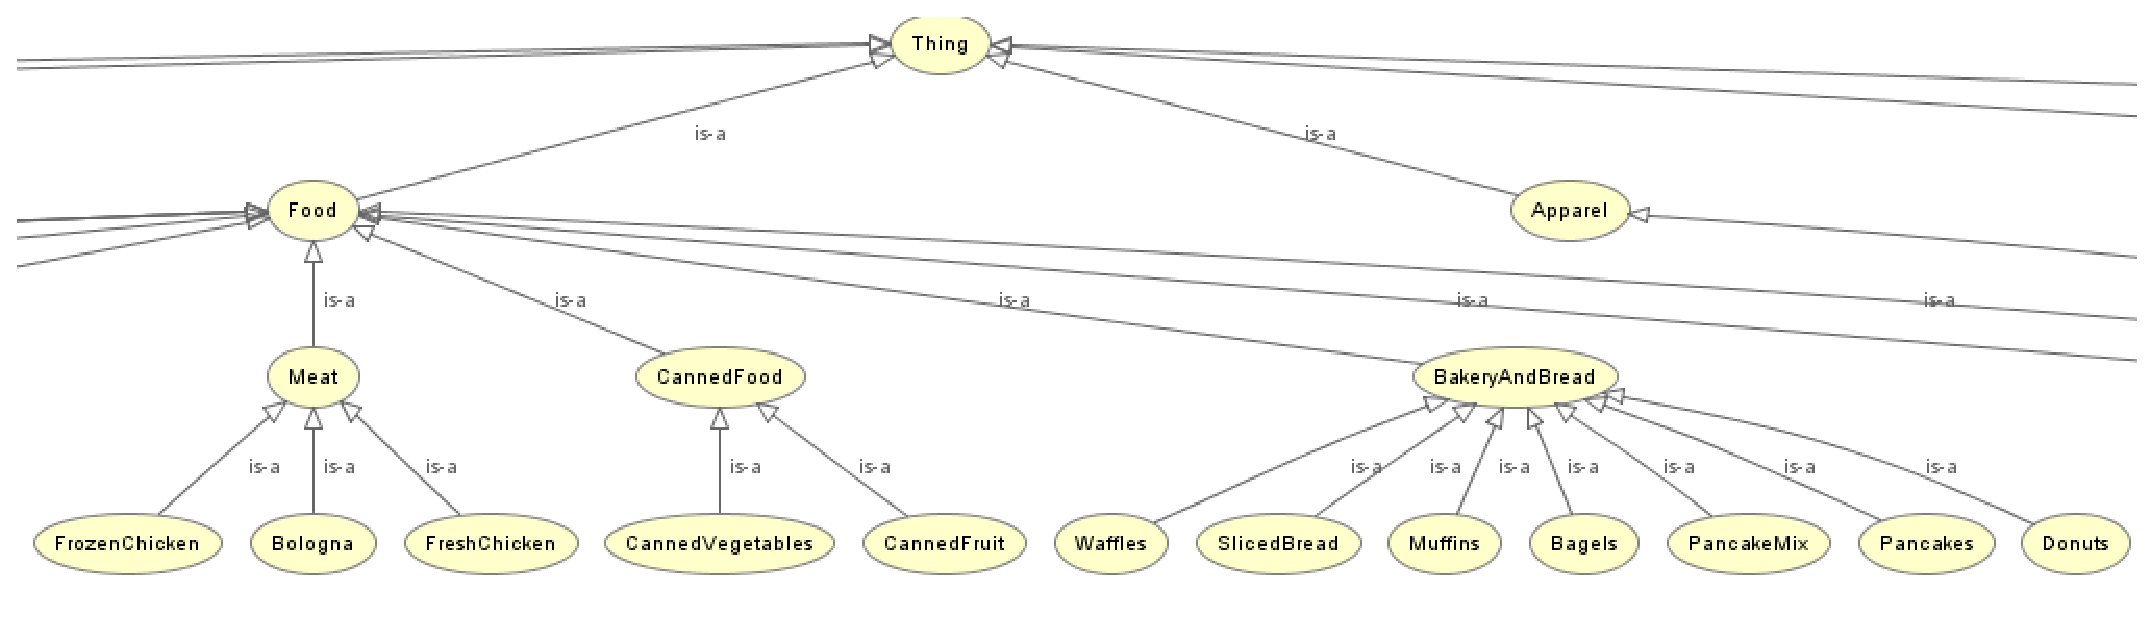
\includegraphics[width=.9\textwidth]{fig/foodmart_onto2.eps}
\end{center}
\caption{\label{fig:foodmart_onto} A portion of the manually created shopping cart ontology.}
\end{figure*}
%
%\subsubsection{Results}
%Items associated with the query term ``toothbrush'' are ranked by the strength of semantic association in Table~\ref{tbl:foodmart_comp}.
%When the ontology is ignored (Table~\ref{tbl:foodmart_comp} (A)), associated items are either hub nodes (with many edges linking to other items) or frequently co-occur with the query item, as in traditional association rule mining over transactional data. Conversely, using only the ontology graph (Table~\ref{tbl:foodmart_comp} (B)) returns the neighborhood of terms in the rdfs:subClassOf lattice. Combining both the ontology and data (Table~\ref{tbl:foodmart_comp} (C--E)),  yields a variety of mixtures of these associations. In a rough sense, it conforms to the ratio of the size of ontology graph and data graph as well (see Table~\ref{tbl:exp_overview}).
%\begin{table*}[tbh]\scriptsize
%\begin{center}
%\begin{tabular}{ c c || c c || c c || c c }
%\hline
%\multicolumn{2}{c||}{$w_o=0$, $w_d=1$}&\multicolumn{2}{c||}{$w_o=1$, $w_d=0$}&\multicolumn{2}{c||}{$w_o=1$, $w_d=1$}&\multicolumn{2}{c}{$w_o=10$, $w_d=1$}    \\
%\hline
%item	&	p(\%)	&	item	&	p(\%)	&	item	&	p(\%)	&	item	&	p(\%)	\\
%\hline															
%Soup	&	0.42	&	PersonalHygiene	&	12.55	&	PersonalHygiene	&	0.74	&	PersonalHygiene	&	3.97	\\
%Cookies	&	0.41	&	Snack	&	0.86	&	Soup	&	0.41	&	NasalSprays	&	0.41	\\
%NasalSprays	&	0.38	&	Health	&	0.64	&	Cookies	&	0.4	&	Soup	&	0.34	\\
%Popcorn	&	0.32	&	Sponges	&	0.57	&	NasalSprays	&	0.37	&	Cookies	&	0.34	\\
%PaperWipes	&	0.29	&	Soap	&	0.57	&	Popcorn	&	0.31	&	Mouthwash	&	0.3	\\
%FrozenVegetables	&	0.29	&	Shampoo	&	0.57	&	FrozenVegetables	&	0.29	&	Popcorn	&	0.25	 \\
%PersonalHygiene	&	0.26	&	NasalSprays	&	0.57	&	PaperWipes	&	0.28	&	FrozenVegetables	&	0.24	 \\
%DriedFruit	&	0.25	&	Mouthwash	&	0.57	&	DriedFruit	&	0.25	&	PaperWipes	&	0.23	 \\
%Milk	&	0.25	&	Conditioner	&	0.57	&	Milk	&	0.25	&	DriedFruit	&	0.22	\\
%Mouthwash	&	0.24	&	MealCourse	&	0.54	&	Mouthwash	&	0.23	&	Milk	&	0.21	\\
%\hline
%\multicolumn{2}{c}{(A)}  &   \multicolumn{2}{c}{(B)}  &   \multicolumn{2}{c}{(C)}  &   \multicolumn{2}{c}{(D)}  \\
%\end{tabular}
%\end{center}
%\caption{\label{tbl:foodmart_comp} Foodmart items ranked by the strength of semantic association to the query term ``toothbrush.'' The ranking, $p(\%)$, denotes the steady-state probability.}
%\end{table*}
%
%Because we created the ontology to illustrate our point, we filter out all terms exclusive to the ontology in Table~\ref{tbl:foodmart_comp2} to elicit top items associated with the query term ``soup."   The pair \emph{``soup"-``cold remedies"}) (ranked 34th with data graph, not shown in the table) is one that we can find, which makes sense but never co-occurs in the data alone and would not be picked up by traditional methods.
%
%%Finally we tested our methods on the dataset of electronic health records of real patients. This dataset is different from the above two datasets not only in scale but also in practical importance as described in the following.
%% state in very clear sentence what the conclusion is, what is the take-home message you want them to see? xxx
%
%% why is this interesting? what should we have learned? xxx
%
%%finally, lead-in to final experiment... we finally did this last experiment because:  1) its huge, 2) its important to people to solve xxx
%
%\begin{table*}[tbh]\scriptsize
%\begin{center}
%\begin{tabular}{ l r | l r || l r | l r }
%\hline
%\multicolumn{4}{c||}{$w_o=0$, $w_d=1$}  &   \multicolumn{4}{c}{$w_o=1$, $w_d=0$}\\
%\hline
%item	&	p(\%)	&	item	&	p(\%)	&	item	&	p(\%)	&	item	&	p(\%)	\\
%\hline
%Cheese	&	0.38	&	Preserves	&	0.19	&	TVDinner	&	0.46	&	Sponges	&	0.06	\\
%Cookies	&	0.32	&	Juice	&	0.17	&	Pizza	&	0.46	&	Soap	&	0.06	\\
%DriedFruit	&	0.32	&	Lightbulbs	&	0.17	&	Pasta	&	0.46	&	Shampoo	&	0.06	\\
%Wine	&	0.24	&	PaperWipes	&	0.16	&	HotDogs	&	0.46	&	NasalSprays	&	0.06	\\
%CannedVegetables	&	0.23	&	Pizza	&	0.16	&	Hamburger	&	0.46	&	Mouthwash	&	0.06	\\
%FrozenVegetables	&	0.23	&	Nuts	&	0.16	&	FrenchFries	&	0.46	&	Conditioner	&	0.06	\\
%Cereal	&	0.22	&	Popcorn	&	0.16	&	DeliSalads	&	0.46	&	Ibuprofen	&	0.06	\\
%Milk	&	0.22	&	Chips	&	0.16	&	DeliMeats	&	0.46	&	ColdRemedies	&	0.06	\\
%ChocolateCandy	&	0.19	&	Eggs	&	0.16	&	Sunglasses	&	0.07	&	Aspirin	&	0.06	\\
%Waffles	&	0.19	&	TVDinner	&	0.15	&	Toothbrushes	&	0.06	&	Acetominifen	&	0.06	\\					 
%\hline
%\end{tabular}
%\end{center}
%\caption{\label{tbl:foodmart_comp2} Foodmart items ranked by the strength of semantic association to the query term ``soup.'' The ranking, $p(\%)$, denotes the steady-state probability. Terms exclusive to the Foodmart ontology are filtered out.}
%\end{table*}


\subsection{Shopping Cart}
\subsubsection{Dataset}
The shopping cart dataset contains purchase information on 100 grocery items (represented by boolean column headers) for 2,127 shopping orders (corresponding to tuples) from a Foodmart. We first construct an RDF bipartite graph from the dataset by transforming the table to 8481 RDF statements.

Besides, we manually create an ontology to organize the grocery items into a subsumption hierarchy (see Figure~\ref{fig:foodmart_onto} for example). In this process, we introduce 28 parent nodes (the 100 grocery items appeared in the data are mostly at the leaf level) from which derive a total of 127 RDF statements. As the size of this dataset is fairly small, the calculation of similarity ranking for a given term is fast. In the following we highlight the effect of incorporation of ontology by comparing results obtained with and without ontologies.


\subsubsection{Results}
In Table~\ref{tbl:foodmart_comp}, results of items ranked by the strength of semantic association with regard to a query term ``Toothbrush" under various combinations of parameters are demonstrated side-by-side for comparison. We first show the result ranked by co-frequency in Table~\ref{tbl:foodmart_comp}(A) as a baseline. Then, we observe that without using ontology, performing random walk with restart on the data graph (Table~\ref{tbl:foodmart_comp}(A)) starting from ``toothbrush" yields similar results to the work reported in~\cite{LiuEtal11} based on random walk commute time similarity. Items ranked high in this setting where only the data graph is considered are typically either hub nodes (with many edges linking to other items) or co-frequent with the query item (many edges connecting them). Second, applying the same similarity ranking method solely on the ontology graph (Table~\ref{tbl:foodmart_comp}(C)) gives a list of association based on the graph-configuration of the ontological structure (in this case, the rdfs:subClassOf lattice). The items that are considered most similar to the query term ``Toothbrush" is its immediate parent class ``PersonalHygiene," followed by some most derived classes at the same level of ``PersonalHygiene" and then siblings of ``Toothbrush" itself. Next, Table~\ref{tbl:foodmart_comp}(D)--(F) demonstrate the results of mining on the combined graph with different ratios of weights assigned to ontology edges and data edges respectively. It is obvious that these results can be seen as a mix of the data-only and ontology-only results with various emphasis on the data or ontology. We can observe that when $w_o/w_d=20$ the ontology and data appear to have equal significance in determining the ranking ($w_o$ is the weight of ontology edges (i.e., rdfs:subClassOf) and $w_d$ is the weight of data edges). In a rough sense, it conforms to the ratio of the size of ontology graph and data graph as well (see Table~\ref{tbl:exp_overview}). In reality, the appropriate ratio for the edge weights is not only dependent on the size of graphs but also the specific configuration of the graph (depth, average degree, etc). Moreover, specifying the ratio of prior knowledge in ontologies and inductive evidences in data that one wants to employ for discovering new patterns is a highly empirical process. Multiple pilot trials may need to be carried out for the optimal ratio before it is applied to the real application.

\begin{table*}[tbh]\scriptsize
\begin{center}
\begin{tabular}{ c c || c c | c c }
\hline
\multicolumn{2}{c||}{ranked by co-frequency}&\multicolumn{2}{c|}{w/ data only}&\multicolumn{2}{c}{w/ ontology only}\\
\hline
item	&	freq	&	item	&	p(\%)	&	item	&	p(\%)	\\
\hline											
PaperWipes	&	8	&	Soup	&	0.42	&	PersonalHygiene	&	12.55	\\
Popcorn	&	7	&	Cookies	&	0.41	&	Snack	&	0.86	\\
Soup	&	6	&	NasalSprays	&	0.38	&	Health	&	0.64	\\
NasalSprays	&	6	&	Popcorn	&	0.32	&	Sponges	&	0.57	\\
Cookies	&	6	&	PaperWipes	&	0.29	&	Soap	&	0.57	\\
Spices	&	5	&	FrozenVegetables	&	0.29	&	Shampoo	&	0.57	\\
Soda	&	4	&	PersonalHygiene	&	0.26	&	NasalSprays	&	0.57	\\
Shrimp	&	4	&	DriedFruit	&	0.25	&	Mouthwash	&	0.57	\\
FlavoredDrinks	&	4	&	Milk	&	0.25	&	Conditioner	&	0.57	\\
Dips	&	4	&	Mouthwash	&	0.24	&	MealCourse	&	0.54	\\
\hline
\multicolumn{6}{c}{~}\\
\multicolumn{2}{c}{(A)}  &   \multicolumn{2}{c}{(B)}  &   \multicolumn{2}{c}{(C)}  \\
\multicolumn{6}{c}{~}\\
\end{tabular}

\begin{tabular}{ c c | c c | c c }
\hline
\multicolumn{2}{c|}{$w_o=1$, $w_d=1$}&\multicolumn{2}{c|}{$w_o=10$, $w_d=1$}&\multicolumn{2}{c}{$o_w=20$, $o_d=1$}\\
\hline
item	&	p(\%)	&	item	&	p(\%)	&	item	&	p(\%)	\\
				\hline							
PersonalHygiene	&	0.74	&	PersonalHygiene	&	3.97	&	PersonalHygiene	&	6.27	\\
Soup	&	0.41	&	NasalSprays	&	0.41	&	NasalSprays	&	0.5	\\
Cookies	&	0.4	&	Soup	&	0.34	&	Mouthwash	&	0.41	\\
NasalSprays	&	0.37	&	Cookies	&	0.34	&	Shampoo	&	0.31	\\
Popcorn	&	0.31	&	Mouthwash	&	0.3	&	Soup	&	0.29	\\
FrozenVegetables	&	0.29	&	Popcorn	&	0.25	&	Cookies	&	0.29	\\
PaperWipes	&	0.28	&	FrozenVegetables	&	0.24	&	Sponges	&	0.28	\\
DriedFruit	&	0.25	&	PaperWipes	&	0.23	&	Health	&	0.27	\\
Milk	&	0.25	&	DriedFruit	&	0.22	&	Conditioner	&	0.27	\\
Mouthwash	&	0.23	&	Milk	&	0.21	&	Soap	&	0.25	\\
\hline
\multicolumn{4}{c}{~}\\
\multicolumn{2}{c}{(D)}  &  \multicolumn{2}{c}{(E)}  & \multicolumn{2}{c}{(F)}\\
\end{tabular}
\end{center}
\caption[Top results on the Foodmart dataset]{\label{tbl:foodmart_comp} Foodmart items ranked by the strength of semantic association  (i.e., $p(\%)$, the steady-state probability), given the query term ``Tooth Brush."}
\end{table*}

We notice that without any filtering on the ranked semantic associations from the combined graph, the list includes items that never appear in the transactional data. This is because typically the semantic annotation process links table attributes to their most specific matching concept in the ontology which are close to the leaf level. The incorporation of ontology is to aid the mining process, therefore including in the result those parent nodes (e.g.,, ``PersonalHygiene") that never appear in the data is counterintuitive. To overcome this, we can simply filter out those items exclusive to the ontology. Table~\ref{tbl:foodmart_comp2} shows an example of filtered result given a query term ``soup." The co-frequency of items are also listed for comparison.

%Finally we tested our methods on the dataset of electronic health records of real patients. This dataset is different from the above two datasets not only in scale but also in practical importance as described in the following.
% state in very clear sentence what the conclusion is, what is the take-home message you want them to see? xxx

% why is this interesting? what should we have learned? xxx

%finally, lead-in to final experiment... we finally did this last experiment because:  1) its huge, 2) its important to people to solve xxx

\begin{table*}[tbh]\scriptsize
\begin{center}
\begin{tabular}{ c c c | c c c |}
\hline											
\multicolumn{6}{c|}{w/ data only}\\											
\hline											
item	&	p(\%)	&	freq	&	item	&	p(\%)	&	freq	 \\
\hline											
Cheese	&	0.38	&	98	&	Preserves	&	0.19	&	65	 \\
Cookies	&	0.32	&	96	&	Juice	&	0.17	&	47	\\
DriedFruit	&	0.32	&	87	&	Lightbulbs	&	0.17	&	47	 \\
Wine	&	0.24	&	63	&	PaperWipes	&	0.16	&	55	 \\
CannedVegetables	&	0.23	&	67	&	Pizza	&	0.16	&	46	 \\
FrozenVegetables	&	0.23	&	79	&	Nuts	&	0.16	&	60	 \\
Cereal	&	0.22	&	56	&	Popcorn	&	0.16	&	39	 \\
Milk	&	0.22	&	53	&	Chips	&	0.16	&	46	 \\
ChocolateCandy	&	0.19	&	16	&	Eggs	&	0.16	&	51	 \\
Waffles	&	0.19	&	51	&	TVDinner	&	0.15	&	40	 \\
\hline									
\end{tabular}
\begin{tabular}{ | c c c | c c c }
\hline									
\multicolumn{6}{|c}{w/ onto only}\\											
\hline
item	&	p(\%)	&	freq	&	item	&	freq	&	 p(\%)	 \\
\hline
TVDinner	&	0.46	&	40	&	Sponges	&	21	&	0.06	 \\
Pizza	&	0.46	&	46	&	Soap	&	0	&	0.06	\\
Pasta	&	0.46	&	29	&	Shampoo	&	34	&	0.06	 \\
HotDogs	&	0.46	&	30	&	NasalSprays	&	21	&	0.06	 \\
Hamburger	&	0.46	&	19	&	Mouthwash	&	28	 &	0.06	 \\
FrenchFries	&	0.46	&	37	&	Conditioner	&	12	 &	0.06	 \\
DeliSalads	&	0.46	&	31	&	Ibuprofen	&	18	&	0.06	 \\
DeliMeats	&	0.46	&	37	&	ColdRemedies	&	33	&	0.06	 \\
Sunglasses	&	0.07	&	12	&	Aspirin	&	22	&	0.06	 \\
Toothbrushes	&	0.06	&	13	&	Acetominifen	&	12	 &	0.06	 \\
\hline
\end{tabular}
\end{center}
\caption[Top results on the Foodmart dataset excluding concepts only in\protect\newline the ontology]{\label{tbl:foodmart_comp2} Semantically associated items  for the query term ``Soup," by filtering out those items exclusive to the Foodmart ontology.}
\end{table*}


\subsection{Electronic Health Records}
\subsubsection{Dataset}
In our second evaluation, we analyzed the electronic health records of real patients. The patient clinical note data are from Stanford Hospital's Clinical Data Warehouse (STRIDE). These records archive over 17-years worth of patient data comprising of 1.6 million patients, 15 million encounters, 25 million coded ICD9 diagnoses, and a combination of pathology, radiology, and transcription reports totaling over 9 million clinical notes (i.e., unstructured text).
We obtained the set of drugs and diseases for each patient's clinical note by using a new tool, the \emph{Annotator Workflow}, developed at the National Center for Biomedical Ontology (NCBO), which annotates clinical text from electronic health record systems and extracts disease and drug mentions from the electronic health records.

%In addition to having obvious data-mining applications, the workflow has been used by biomedical researchers to build semantic-search applications, such as the NCBO Resource Index~\cite{jonquet11}, which won the Semantic Web Challenge\footnote{\url{http://challenge.semanticweb.org/}} in 2010. The annotation process utilizes the vast NCBO BioPortal ontology library~\cite{bioportal} to extract information by using a lexicon of over one million terms generated from the relevant ontologies, such as SNOMED-CT, RxNORM, and MedDRA. Furthermore, it also incorporates negation detection --- the ability to discern whether a term is negated with the context of the narrative (e.g., lack of valvular dysfunction). Finally, it uses mappings between terms across ontologies~\cite{ghazvinian09}, which forms a rich knowledge graph %(Figure~\ref{fig:collapse})
%or mega-thesaurus, to normalize the lexicon by reducing the feature set from over one million to merely 11,107 unique drugs and 3,594 unique diseases.

From this set of 1.6 million patients with annotated records, we vectorize texts and turned them into a huge bag-of-word representation, from which an RDF bipartite graph is constructed (including 148 million RDF statements, see Table~\ref{tbl:exp_overview}). we applied our algorithms to all previous records in the patient's timeline, looking at just the set of drugs and their semantically related diseases.  Therefore, at a very simplistic level, the experiment result shows that strong semantically associated items in this context could possibly represent sets of drugs that could lead toward certain diseases.

One strength of the Annotator is the highly comprehensive and interlinked lexicon that it uses. It can incorporate the entire NCBO BioPortal ontology library of over 250 ontologies to identify biomedical concepts from text using a dictionary of terms generated from those ontologies. Terms from these ontologies are linked together via mappings. For this study, we specifically configured the workflow to use a subset of those ontologies that are most relevant to clinical domains, including Unified Medical Language System (UMLS) terminologies such as SNOMED-CT, the National Drug File (NDFRT) and RxNORM, as well as ontologies like the Human Disease Ontology. The resulting set of ontologies contains 1 million subsumption statements.

To highlight the capability of our method for incorporating multiple types of relationships, we also explore the ``may\_treat" relationship between drugs and diseases defined in NDFRT, for example, Thiabendazole may\_treat Larva Migrans. Since we are interested in learning the interaction between drugs and diseases, may\_treat is naturally a better indicator relationship to include while mining semantic associations than the subsumption relationship. Our results below illustrate this point.


\subsubsection{Results}
Before studying the drug-disease association, we carried out a similar test to that on the shopping cart dataset, in which we focus on studying the drug-drug and disease-disease association. To this purpose, we combine the subsumption hierarchy in the ontology graph with the data graph. Table~\ref{tbl:health_comp} shows the ranked semantic association for the query term ``Rofecoxib" (an active ingredient of some anti-inflammatory drugs) given different weight configuration to combine graphs. Without any preprocessing and prior knowledge about how the clinical notes are prescribed, the incorporation of subsumption relationship can be seen as a mean for denoising and enhancement of the data. Given the ratio of the size of the ontology to the size of data, the data graph in this test is more dominant in determining the ranking than in the shopping cart experiment. One can gradually change the ratio of $w_o$ to $w_d$ to strike a balance and achieve the optimal result.
\begin{table*}[tbh]\scriptsize
\begin{center}
\begin{tabular}{ c | c | c | c  }
\hline
rank    &   w/ data only	&	w/ onto only		&$w_o=10000, w_d=1$	 \\
\hline
1	&		reflux	&	valdecoxib	&		reflux	\\
2	&		medical history	&	meloxicam	&		obstruction	\\
3	&		history of previous events	&	celecoxib	&		injury	\\
4	&		diagnosis	&	parecoxib	&		valdecoxib	\\
5	&		pharmaceutical preparations	&	etoricoxib	&		medical history	\\
6	&		blood and lymphatic system disorders	&	deracoxib	&		foreign body sensation	\\
7	&		disease	&	lumiracoxib	&		history of previous events	\\
8	&		infantile neuroaxonal dystrophy	&	firocoxib	&		adverse effects	\\
9	&		today	&	nabumetone	&		celecoxib	\\
10	&		hypersensitivity	&	macrolides	&		actual hypothermia	\\
\hline
\end{tabular}
\end{center}
\caption[Top results on the electronic health dataset]{\label{tbl:health_comp}Results of Health items ranked by the strength of semantic association, given the query term ``Rofecoxib."}
\end{table*}

To verify the drug--disease association and study the impact of different semantic relationships on finding such association, we carry out the following experiment. Table~\ref{tbl:health_exp} illustrates the rankings of three associations (one per row) under different settings. The first element in the pair is the query item, which are all active ingredients of some prescription drugs, and the ranking shown in the table is for the second item, which are diseases. For example, arthritis is ranked as the 527th semantically associated item to Rofecoxib according to similarity ranking based only on data graph. All these item pairs are actually gold standard associations backed by known drug--disease relationships, we know the strength of semantic associations between them should be strong.

We observe that the ranking based on data graph alone is fairly high already, consider there are approximately 1 million concepts of interest. However, the results based on the combination of data and subsumption (``isa") graph are worse. It is because the subsumption hierarchies for drugs and diseases are largely separate structures. Therefore the subsumption relationships can only boost the association within the drug and disease hierarchies respectively, but obfuscate the cross-hierarchy associations that we aim to find between drugs and diseases. On the other hand, however, the association between these pairs can be exactly captured by the NDFRT ``may\_treat" relationship (e.g.,, NDFRT explicitly defines that Rofecoxib may\_treat arthritis). When the ``may\_treat" graph is incorporated into the mining process, the ranking for the association is greatly boosted.

\begin{table*}[tbh]\scriptsize
\begin{center}
\begin{tabular}{ c || c  c || c  c || c  c }
\hline
        &   \multicolumn{2}{c||}{w/ data only}  &   \multicolumn{2}{c||}{w/ data and ``isa"} & \multicolumn{2}{c}{w/ data and ``may\_treat"}\\
\hline
\hline
                        	&   p(\%)   &   rank    &   p(\%)    &   rank    &   p(\%)    &    rank    \\
\hline
$\langle Rofecoxib, degenerative~polyarthritis\rangle$  &   0.006   &   527     &   0.004    &   632     &   0.51     &     13     \\
$\langle valdecoxib, degenerative~polyarthritis\rangle$  &   0.007   &   613     &   0.005    &   695     &   0.63     &     17     \\
$\langle troglitazone, diabetes\rangle$  &   0.006   &   478     &   0.005    &   514     &   0.44     &     11     \\
\hline
\end{tabular}
\end{center}
\caption[Rankings of three semantic associations in health data under\protect\newline different settings]{\label{tbl:health_exp}Rankings of three semantic associations in health data under different settings.}
\end{table*}





\begin{figure}[tbh]
\begin{minipage}[c]{0.49\textwidth}\centering
\includegraphics[width=.52\textwidth]{fig/may_treat.eps}
\end{minipage}
\begin{minipage}[c]{0.49\textwidth}\centering
\includegraphics[width=.72\textwidth]{fig/may_treat_augmented.eps}
\end{minipage}
\caption[The may\_treat subgraph]{\label{fig:may_treat} The may\_treat subgraph before and after distortion: The left-hand side of the figure shows the may\_treat subgraph of ground truth relationships between the drug Rofecoxib and two diseases. The right-hand side shows the may\_treat subgraph with some deliberately distorted information.}
\end{figure}

\begin{table*}[tbh]\scriptsize
\begin{center}
\begin{tabular}{ c || c  c || c  c }
\hline
        &   \multicolumn{2}{c||}{w/ noisy may\_treat only}    &   \multicolumn{2}{c}{w/ data and noisy may\_treat}\\
\hline
\hline
       	&   p(\%)   &   rank    &  p(\%)    &    rank    \\
\hline
$\langle Rofecoxib, degenerative~polyarthritis\rangle$       &   3.60e-3   &   555     &   8.14e-3    &   263    \\
$\langle Rofecoxib, dysmenorrhea\rangle$    &   1.54e-2   &   246     &   1.26e-3    &   1703   \\
\hline
\end{tabular}
\end{center}
\caption[Rankings of associations on the noisy may\_treat graph]{\label{tbl:salted_may_treat}Rankings of associations on the noisy may\_treat graph (Figure~\ref{fig:may_treat} right) between Rofecoxib and two diseases derived with and without data.}
\end{table*}

Conversely, we are also interested in learning whether the data graph can help discover patterns in the ontology graph. Figure~\ref{fig:may_treat} (left) shows a subgraph of the NDFRT ``may\_treat" relationship. Rofecoxib is asserted to treat two diseases, namely, dysmenorrhea and degenerative polyarthritis. And there are altogether 116 and 200 drugs that are known to treat dysmenorrhea and degenerative polyarthritis respectively (hence the in-degrees of the nodes). Applying our method on this graph with the query term ``Rofecoxib" yields a similarity-ranked list having degenerative polyarthritis and dysmenorrhea as the top two items. Since this result is the exact ground truth, there is no improvement to be made with the incorporation of the data graph. Therefore, we alter the ground truth graph with some deliberately distorted information, as is shown in Figure~\ref{fig:may_treat} (right), so that the may\_treat graph alone produces only inferior result. More specifically, we specify that Rofecoxib should treat hypertensive disease, the very diseases that is asserted to be treated by the most drugs (a total of 619). Then we add an imaginary drug to treat degenerative polyarthritis, dysmenorrhea, and hypertensive disease. In this way, the original direct connections between Rofecoxb and degenerative polyarthritis and dysmenorrhea become erroneously indirect and are obfuscated by some the noise of high degree nodes along the path. With this scenario, we hope to learn if the incorporation of data graph can correct the misinformation in ontologies.

Table~\ref{tbl:salted_may_treat} shows the result of ranks of the associations between Rofecoxib and degenerative polyarthritis and dysmenorrhea. The ranks of the associations drastically drop to the 555th and 246th respectively on the noisy graph from the top two on the original ground truth graph. This is mainly due to the large node, hypertensive disease, in the middle of the connections. However, with the combined data and may\_treat graph, we notice that the rank of Rofecoxib and degenerative polyarthritis increases to 263rd, while the rank of Rofecoxib and  dysmenorrhea decreases to 1703rd. This shows that the data graph endorses more strongly the association between Rofecoxib and degenerative polyarthritis. Indeed, although Rofecoxib are known to treat both degenerative polyarthritis and dysmenorrhea, the former is a much more popular usage. A search on the National Library of Medicine's PubMed database\footnotemark[1] for ``Rofecoxib and polyarthritis" returns 518 results, while ``Rofecoxib and dysmenorrhea" only returns 29. This result shows that the data graph can help correct misinformation in ontologies to some extent, and in a sense, it also gives a clue of how prior beliefs fit with reality.

\footnotetext[1]{\url{http://www.ncbi.nlm.nih.gov/}}


\section{Discussion}
\label{sec:discussion}
We have demonstrated that using the proposed combined RDF bipartite graph incorporates both domain knowledge and data based on the user's desired weights for each component for finding \emph{semantically associated itemsets}.

Developing scalable algorithms for semantic data mining is critically important. In our work, the healthcare dataset has grown beyond 100 billion triples and the size of the ontologies used are also large (SNOMED-CT has nearly 400,000 classes). The RWR method we describe works well for query-based node similarity, but it will not scale to generate full pair-wise node similarities at this tremendous scale because a calculation of eigenvectors of the Laplacian is required to derive the similarity measures, which is very expensive on large graphs.

While non-trivial practical problems associated with very large graphs cannot be completely avoided, our work makes it possible to leverage decades of work on graph-based methods in this effort to mine semantically associated data. The general strategy going forward is to employ approximation and develop parallelizable algorithms. Lin and Cohen~\cite{LinEtal2010ICML} proposed an approximation to a eigenvalue-weighted linear combination of all the eigenvectors, which can be achieved by performing a small number of matrix-vector multiplications.  The procedure results in a more scalable method called \emph{power iteration clustering} that finds a very low-dimensional data embedding using truncated power iteration on a normalized pair-wise similarity matrix of the data points. Zhao et al.~\cite{ZhaoEtal2011Eff} described the idea of \emph{graph coordinate systems}, which provides a fast embedding of large graphs into a hyperbolic space. The method parallelizes easily and efficiently locate shortest paths between node pairs, which relates well to the notion of commute time distance, which our RWR method seeks to elicit. Savas and Dhillon~\cite{SavasEtal2011Clu} introduced a novel framework called \emph{clustered low rank matrix approximation for massive graphs}. After a few intermediate steps, they are able to finally project an a optimal, low rank approximation of the entire graph, thus including connections or edges between vertices from different clusters. We intend to extend these ideas to ontology-annotated hypergraphs.

The weighted hyperedges provide a great deal of flexibility to users who may prefer domain knowledge over data (or vice versa) and opens up new research questions on how to optimally configure learning algorithms. In reality, the appropriate ratio for the edge weights is not only dependent on the size of graphs but also the graph configuration (depth, average degree, etc). Moreover, allowing users to specify the ratio of prior knowledge in ontologies versus inductive evidence from data enables us to discover empirically optimal configurations. We have performed exhaustive feature selection on classification algorithms for our healthcare dataset in the past, and we would also explore a few permutations on these hyperedge weights going forward. We can draw upon other works, such as, Tian et al.~\cite{Tian2009AHyper}, who proposed a semi-supervised approach for classifying nodes in a graph based on a relatively small labeled set.

The RDF bipartite graph representation has limited expressivity compared to OWL itself. For example, domain, range and cardinality constraints are not straightforward to model.  One possible approach is to model domain constraints by explicitly describing the desired or acceptable walk (traversal sequence) in the RDF hypergraph. In this case, the recently proposed \emph{regular traversal expression} ~\cite{Marko10} technique may apply. However, their fast power-iteration approach for computing the stationary probability may not be applicable any more due to the label sequence constraint, but the Monte-Carlo simulation of the random walk may help to approximate the similarity measure.

We have showcased the utility of the RDF bipartite graph in mining \emph{semantically associated itemsets} and will explore other data mining tasks as well. For example, the the classification task can be formulated as discovering the correct labels for unlabeled vertices in the weighted bipartite graph. Conceptually, the pair of nodes being ``close to'' one another shall share the same labels, which are consistent to one basic principle of semi-supervised learning, so the challenge is to define the closeness between two nodes. The clustering task can be viewed as a neighborhood formation for vertices on the data partition. Basically, for any closely related nodes, we group them together. Again, with an explicit similarity measure, possibly even the classical k-means in this case, could be directly applied to cluster the vertices. 
\section{Conclusion and Future Work}
\label{sec:conclusion}

%We approach the discovery of indirectly associated items from ontology-annotated data, called \emph{semantically associated itemsets}, by proposing a new semantic data mining technique.  Our method uses hypergraphs and random walks with restart over a bipartite graph serialization to discover associations that cannot be found by methods that rely on co-frequent items because it utilizes both the ontology and the data at the same time.  Moreover, we allow users the ability to customize the weight of each component, giving flexibility in how strongly the role of the ontology plays over the data, or vice-versa.  Our evaluations show that the method discovers indirect associations and that it scales to datasets that are large in multiple says: the ontology can be large and the data can be large.
%
%In future work, we will explore algorithms that suggest appropriate weights to apply to the components of the hypergraph. Also, we will implement methods for clustering and classification tasks within this framework. We will focus on our healthcare datasets mainly because they are both large and complex, but also because of the enormous potential in advancing the state-of-the-art in clinical informatics and improving the quality of care for millions of patients.

We mine biomedical ontologies and  data using a unified RDF hypergraph representation.  Our method uses random walks with restart over a bipartite graph serialization to discover semantic (indirect) associations that cannot be found by methods that rely on co-frequencies because our method utilizes both the ontology and the data at the same time. We are one of the first research groups which consider to mine biomedical ontologies and data together without using a separate system to pre-processing or pre-computing ontologies. We allow users the ability to customize the weight of each component, giving flexibility in how strongly the role of the ontology plays over the data, or vice-versa.  Our evaluations show that the method discovers semantic associations and that it scales to datasets that are large in multiple says: the ontology can be large and the data can be large. Moreover, we also show that our data mining methods can discover the errors in biomedical ontologies injected by human operations.

In the following we highlight some future research directions in mining the unified RDF bipartite graph.

Developing scalable algorithms for semantic data mining is critically important. The healthcare dataset in our study has grown beyond 100 billion triples and the size of the ontologies used are also large (SNOMED-CT has nearly 400,000 classes). The RWR method we describe works well for query-based node similarity, but it will not scale to generate full pair-wise node similarities at this tremendous scale because a calculation of eigenvectors of the Laplacian is required to derive the similarity measures, which is very expensive on large graphs. While non-trivial practical problems associated with very large graphs cannot be completely avoided, our work makes it possible to leverage decades of work on graph-based methods in this effort to mine semantically associated data. A promising direction going forward is to employ approximation and develop parallelizable algorithms.

The weighted hyperedges provide a great deal of flexibility to users who may prefer domain knowledge over data (or vice versa) and opens up new research questions on how to optimally configure learning algorithms. In reality, the appropriate ratio for the edge weights is not only dependent on the size of graphs but also the graph configuration (depth, average degree, etc). Moreover, allowing users to specify the ratio of prior knowledge in ontologies versus inductive evidence from data enables us to discover empirically optimal configurations. We have performed exhaustive feature selection on classification algorithms for our healthcare dataset in the past, and we would also explore a few permutations on these hyperedge weights going forward.

The RDF bipartite graph representation has limited expressivity compared to OWL itself. For example, domain, range and cardinality constraints are not straightforward to model.  One possible approach is to model domain constraints by explicitly describing the desired or acceptable walk (traversal sequence) in the RDF hypergraph. In this case, the recently proposed \emph{regular traversal expression} ~\cite{Marko10} technique may apply. However, their fast power-iteration approach for computing the stationary probability may not be applicable any more due to the label sequence constraint, but the Monte-Carlo simulation of the random walk may help to approximate the similarity measure.

We will continue to focus on healthcare datasets mainly because large number of biomedical ontologies have been developed and used to annotate the real-life data, but also because of the enormous potential in advancing the state-of-the-art in clinical informatics and improving the quality of care for millions of patients. This research also contributes to an emerging research direction of semantic data mining, in which formal semantics that exist in data and knowledge can be represented and incorporated into the data mining process in a seamless way.





%ACKNOWLEDGMENTS are optional
%\input{Acknowledgments}

\bibliographystyle{abbrv}
\bibliography{dou,prop,thesis,paea}



\end{document}
